\documentclass[UTF8,a4paper,10pt]{article}
\usepackage{geometry}
% 设置上下左右的页边距
\geometry{left=2cm,right=2cm,top=2cm,bottom=2cm}

\usepackage{ctex}
\usepackage{amsthm}
\usepackage{graphicx}
\usepackage{float}
\usepackage{tabularx} % 加载tabularx宏包
\usepackage[subfigure,AllowH]{graphfig} 

% chktex-file 44

\newtheorem{question}{Question}

\newenvironment{solution}
  {\begin{proof}[Answer]}
  {\end{proof}}

\title{第一章:数据库基础概念作业}
\author{梁昱桐 2100013116}

\begin{document}
	\maketitle 

	\begin{question}
	谈谈你对数据独立性的理解。数据库系统是从哪些方面来提高数据独立性的?
	\end{question}
	
	\begin{solution}
	数据独立性:当数据结构发生变化时,通过系统提供的映象(转换)功能,使应用程序不必改变

	我对此的理解是:这反映了应用程序与数据存储和数据访问的隔离程度,所以一个高度数据独立的系统允许修改数据库的结构而不影响使用该数据的应用程序。

	数据库系统主要通过物理独立性和逻辑独立性来提高数据独立性:
	\begin{enumerate}
		\item \textbf{数据的物理独立性}:当数据存储结构发生变化时,使应用程序不必改变
		\item \textbf{数据的逻辑独立性}:当数据逻辑结构发生变化时,使应用程序不必改变
	\end{enumerate}

	具体来讲有以下举措:
	\begin{enumerate}
		\item 把数据库定义和描述从应用程序中分离出去
		\item 数据描述是分级的(全局逻辑、局部逻辑、存储)
		\item 数据存取由系统管理,用户不必考虑存取路径等细节,从而简化了应用程序(SQL)
	\end{enumerate}

	\end{solution}

	\begin{question}
	比较数据库系统和文件系统在数据管理方面的不同,列出至少四个不同之处(可以做一个表格来展示)  
	\end{question}

	\begin{solution}
	下表列出了数据库系统和文件系统在数据管理方面的主要不同之处:

	\begin{table}[H]
	\centering
	\caption{数据库系统与文件系统的比较}
	\begin{tabular}{lll}
	\hline
	\textbf{不同之处} & \textbf{数据库系统} & \textbf{文件系统} \\ 
	\hline
	数据安全性控制 & 提供安全性控制 & 依赖操作系统 \\
	数据完整性控制 & 提供支持 & 依赖应用程序 \\ 
	数据并发控制 & 提供支持 & 依赖应用程序 \\
	数据恢复控制 & 提供支持 & 依赖应用程序 \\
	数据独立性 & 高,由系统提供 & 低,依赖应用程序 \\
	数据共享 & 容易实现数据共享 & 数据共享较困难 \\ 
	数据访问 & 提供复杂的查询语言 & 直接访问或通过简单API \\ 
	\hline
	\end{tabular}
	\end{table}
	\end{solution}

	\begin{question}
	列举两个不适合使用数据库而应该基于文件系统的应用,并给出简单的解释
	\end{question}

	\begin{solution}
		两个不适合使用数据库而应该基于文件系统的应用:

	\begin{enumerate}
		\item \textbf{日志存储}:大量日志数据的写入操作,特别是在高吞吐量的环境下。使用文件系统直接写入日志文件通常更为高效,便于快速追加数据且易于后续处理和分析。
		\item \textbf{小型、低复杂性项目}:对于小型项目,快速迭代和简单性往往比扩展性和数据独立性更重要。在这种情况下,文件系统提供了一种简单、无需额外依赖的数据存储方法。
	\end{enumerate}
	\end{solution}

	\begin{question}
	对不同模型(层次、网状、关系、面向对象模型)从模型结构、表达能力、数据独立性、操作简便性等方面比较其不同(也可以做一个表格来展示) 
	\end{question}

	\begin{solution}
	下表列出了不同模型(层次、网状、关系、面向对象模型)从模型结构、表达能力、数据独立性、操作简便性等方面的比较:

	\begin{table}[H]
	\centering
	\caption{不同模型的比较}
	\begin{tabularx}{\textwidth}{lXXXX}
	\hline
	\textbf{模型} & \textbf{模型结构} & \textbf{表达能力} & \textbf{数据独立性} & \textbf{操作简便性} \\ \hline
	层次模型 & 树形结构 & 有限:一对多,或引入虚拟节点 & 具有 & 低:存取、插入、删除\\	\hline

	网状模型 & 图形结构 & 丰富 & 具有 & 低:图结构操作复杂 \\	\hline

	关系模型 & 表格结构 & 丰富 & 具有:用户只需提出“做什么”,无需说明“怎么做” & 高:二维表直观\\	\hline

	面向对象模型 & 对象结构 & 丰富 & 具有 & 高\\ \hline
	\end{tabularx}
	\end{table}

	\end{solution}

	\begin{question}
	如果采用多维数组作为数据模型,它比较适合管理哪些应用场景的数据?(可以从数组的有序性和关系模型集合的无序性角度入手)
	\end{question}

	\begin{solution}
	多维数组作为有序的表示方法,适合管理以下应用场景的数据:

	\begin{enumerate}
		\item \textbf{图像处理}:在图像处理中,图像可以被表示为二维(灰度图)或三维(彩色图,第三维是颜色通道)数组。这里像素值之间的关系是有序的,多维数组能够有效地组织图像数据;关系模型无法直接表示像素之间的空间关系。
		\item \textbf{时间序列数据}:与时间相关的数据往往具有前后关系,多维数组能够有效地组织前后关系;关系模型无法直接表示时间序列数据之间的前后关系。
	\end{enumerate}

	\end{solution}

	
	\begin{question}
	画出数据库三层模式架构图,简单说明一下模式分层的好处
	\end{question}

	\begin{solution}
	数据库三层模式架构图如下:
	\begin{figure}[H]
		\centering
		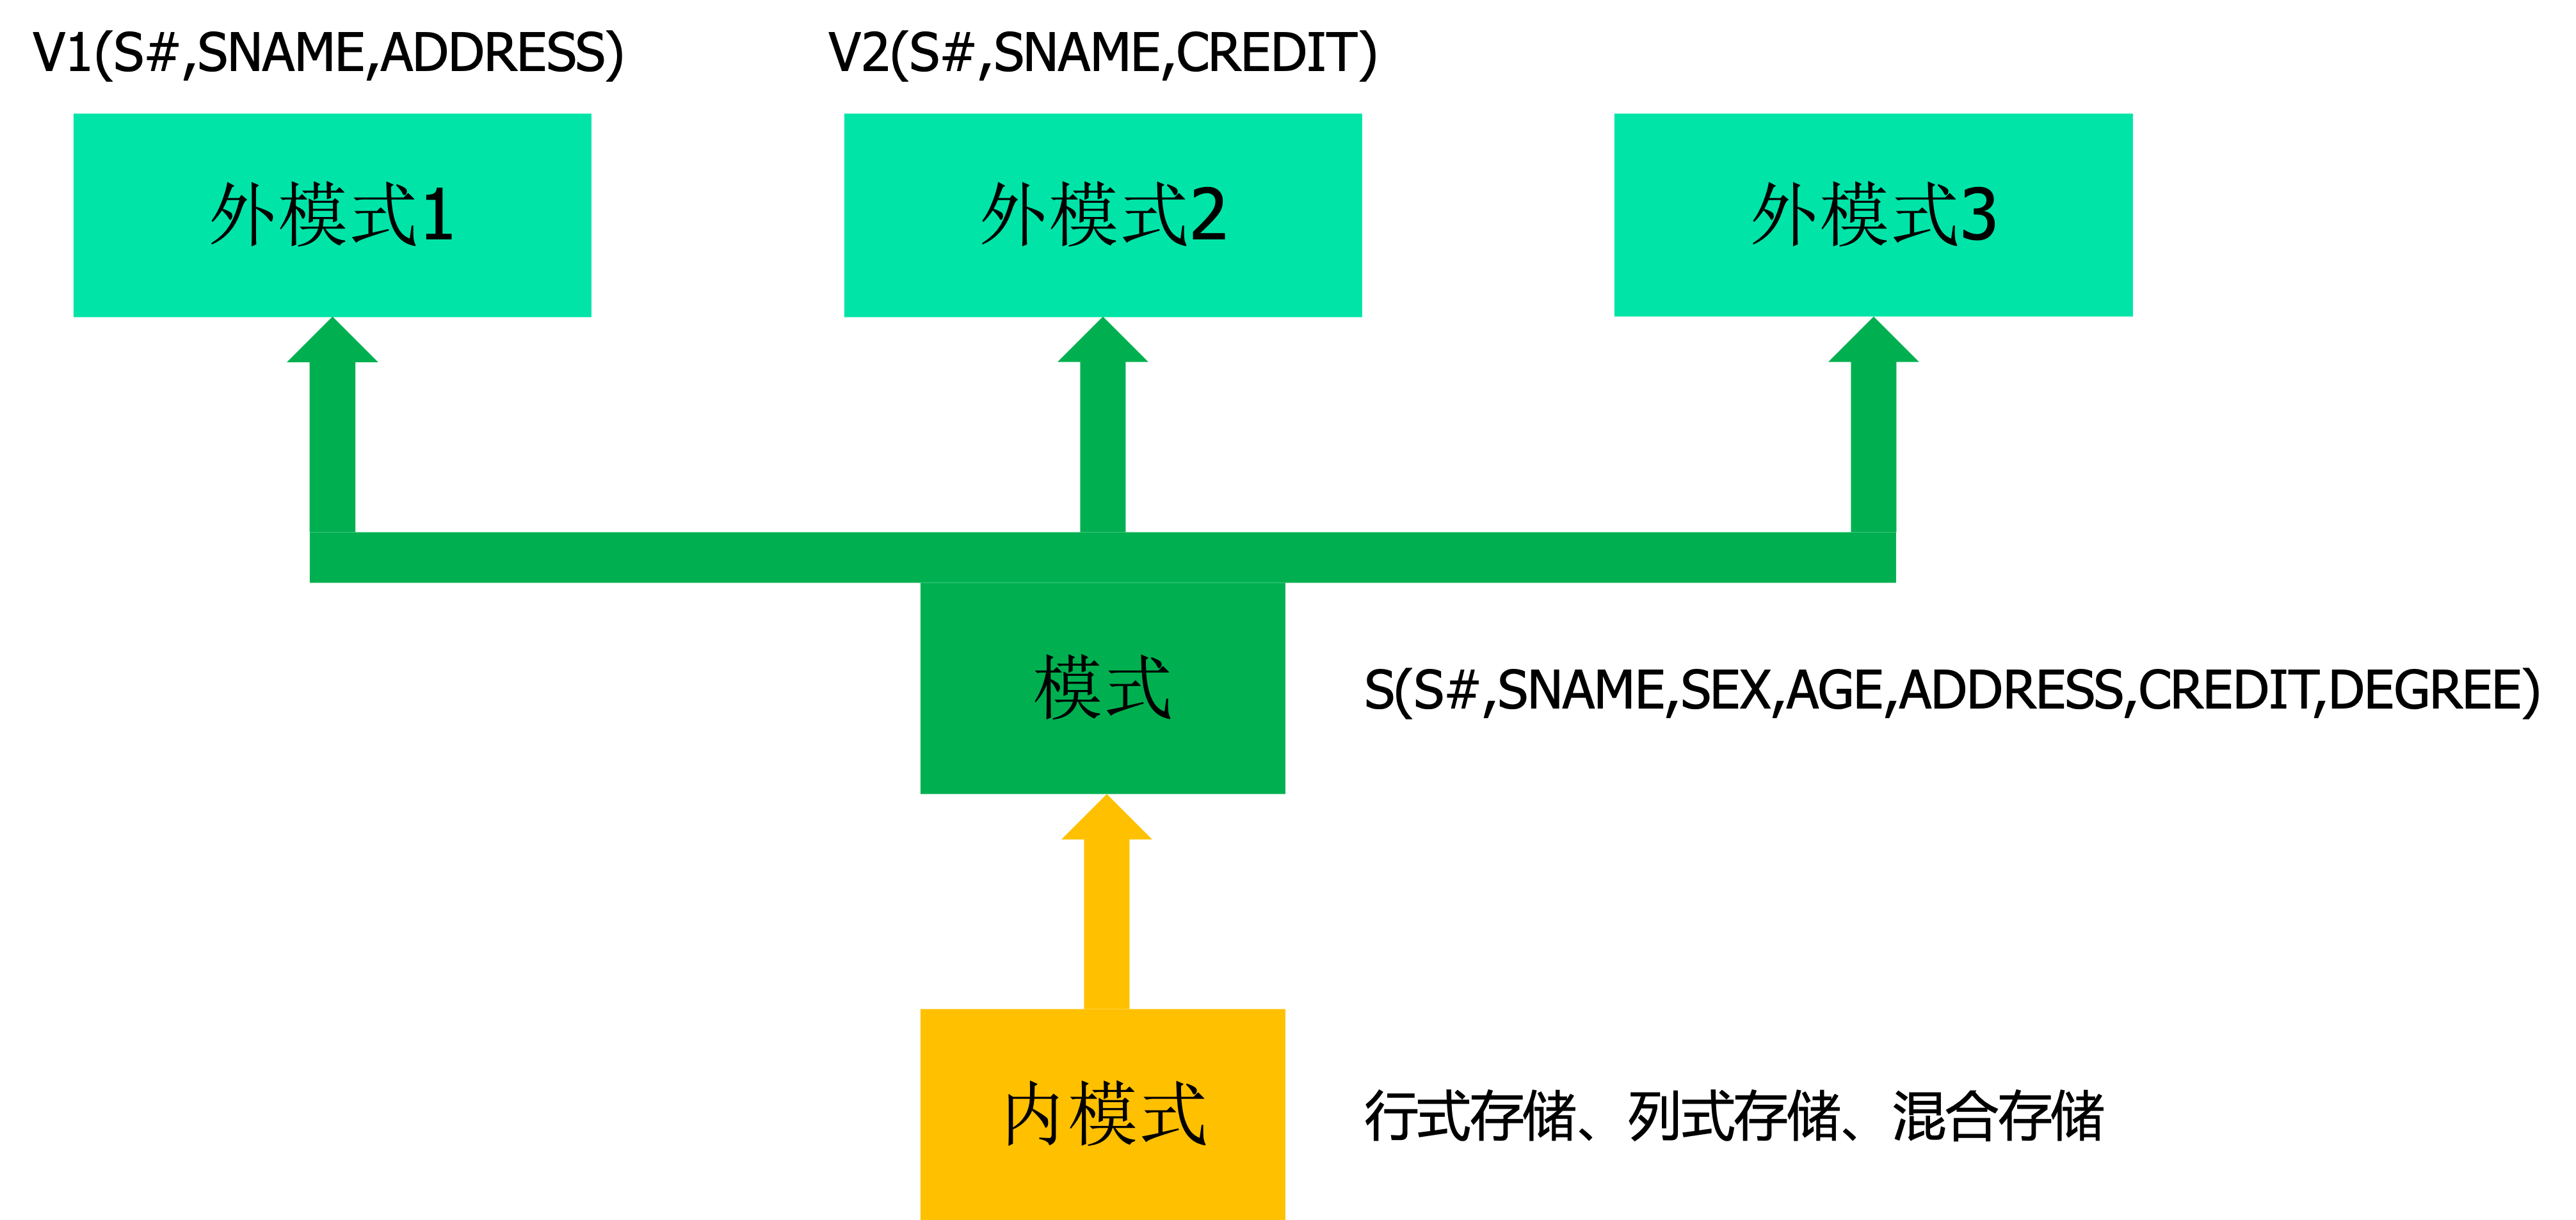
\includegraphics[width=0.8\textwidth]{./fig/three-layer-architecture.png}
		\caption{数据库三层模式架构图}
	\end{figure}

	模式分层的好处:
	\begin{enumerate}
		\item \textbf{外模式和模式之间的对应关系}:当模式改变时,修改外模式/模式映象,使外模式保持不变,从而应用程序可以保持不变,这赋予了数据库以逻辑独立性。
		\item \textbf{逻辑结构与存储结构间的对应关系}:存储结构改变时,修改模式/内模式映象,使模式保持不变,从而应用程序可以保持不变,这赋予了数据库以物理独立性。
	\end{enumerate}

	\end{solution}

	\begin{question}
	搜索引擎的关键字查询和数据库查询有何不同?试从查询方式和查询结果来比较 
	\end{question}

	\begin{solution}区别:
	
	\textbf{查询方式}

	搜索引擎的关键字查询:
	\begin{enumerate}
		\item \textbf{基于文本的搜索}:用户通过输入文字进行查询,搜索引擎会在其索引的网页或文档中查找包含这些关键字的内容。
		\item \textbf{模糊匹配和自然语言处理}:搜索引擎能够处理拼写错误、同义词替换等,通过自然语言处理技术理解用户的查询意图。
	\end{enumerate}

	数据库查询:
	\begin{enumerate}
		\item \textbf{基于查询语言}:数据库查询通常需要使用SQL或其他数据库查询语言编写查询语句,指明要从哪个表中检索什么数据。
		\item \textbf{缺乏自然语言处理能力}:传统数据库查询不处理自然语言查询。
	\end{enumerate}
	
	\textbf{查询结果}
	
	搜索引擎的关键字查询结果:
	\begin{enumerate}
		\item \textbf{非结构化或半结构化数据}:结果通常是网页、文章、图片等非结构化或半结构化的数据。
		\item \textbf{基于相关性的排序}:结果会根据相关性进行排序。
		\item \textbf{可能包含广泛的信息}:搜索引擎旨在从互联网上提供尽可能多的相关信息,结果范围较广。
	\end{enumerate}

	数据库查询结果:
	\begin{enumerate}
		\item \textbf{结构化数据}:结果是以表格形式返回的,每一行代表一个记录,每一列代表一个字段。
		\item \textbf{精确匹配和固定格式的结果}:数据库查询结果基于查询语句的精确条件,返回的所有是满足条件的数据记录。
		\item \textbf{结果范围更为有限和特定}:由于数据库与互联网相比较小,数据库查询的结果通常更加具体和有限。
	\end{enumerate}

	\end{solution}

	\begin{question}
	DBMS的主要数据控制功能应该有哪些?如果有一个淘宝达人想基于单机版数据库比如Access记录自己的购物流水,上面的哪些功能是他所不需要的?
	\end{question}

	\begin{solution}
	DBMS的主要数据控制功能包括:
	\begin{enumerate}
		\item \textbf{安全性控制}:包括用户认证、用户授权、数据加密等。
		\item \textbf{完整性控制}:包括实体完整性、用户定义的完整性等。
		\item \textbf{并发控制}:包括事务管理、锁管理、并发控制等。
		\item \textbf{恢复控制}:包括备份、恢复、日志管理等。
	\end{enumerate}

	淘宝达人基于单机版数据库比如Access记录自己的购物流水时,不需要的功能有:
	\begin{enumerate}
		\item \textbf{并发控制}:单机版数据库不需要考虑并发控制问题,因为只有一个用户在使用。
		\item \textbf{恢复控制}:单机版数据库不需要考虑备份、恢复、日志管理等问题,因为数据量小,且不需要保证高可用性。
	\end{enumerate}

	\end{solution}

	\begin{question}
	DBA应该履行哪些职能?相应的他又应该具备哪些技能?
	\end{question}

	\begin{solution}

	DBA应该履行的职能包括:
	\begin{enumerate}
		\item \textbf{数据库设计}:设计数据库的逻辑结构和物理结构。
		\item \textbf{数据库实施}:安装、配置、调优数据库系统。
		\item \textbf{数据库维护}:监控数据库性能、调整数据库参数、备份和恢复数据库。
		\item \textbf{数据库安全}:管理用户权限、保护数据库安全。
		\item \textbf{数据库规划}:规划数据库的发展方向,包括容量规划、性能规划等。
	\end{enumerate}

	DBA应该具备的技能包括:
	\begin{enumerate}
		\item \textbf{数据库技术}:熟悉数据库系统的原理、架构、SQL语言等。
		\item \textbf{操作系统技术}:熟悉操作系统的原理、架构、命令等。
		\item \textbf{网络技术}:熟悉网络的原理、架构、协议等。
		\item \textbf{安全技术}:熟悉安全技术,包括加密、认证、授权等。
		\item \textbf{管理技术}:熟悉项目管理、团队管理、沟通技巧等。
	\end{enumerate}

	\end{solution}

	\begin{question}
	(选做,不做不扣分,做了不加分)自己尝试从概念上解释一下什么是DB for AI?什么又是AI for DB?可以简单搜索并罗列一些这方面的研究问题或已有工作
	\end{question}

	\begin{solution}
	DB for AI和AI for DB是两个相关但不同的概念:

	\textbf{DB for AI}:“DB for AI”指的是将数据库技术应用于人工智能领域的过程。具体来说,这涉及到如何有效地在数据库中存储、管理和检索大量的数据,以供AI模型训练和推理使用。在这个过程中,数据库不仅仅是静态数据的仓库,而是需要支持高效的数据处理和分析操作,比如时间序列分析、图数据处理、复杂事件处理等。因此,“DB for AI”关注于如何设计和优化数据库系统,以满足AI应用对数据处理的特殊需求。

	\textbf{AI for DB}:“AI for DB”则是指使用人工智能技术来优化和增强数据库系统的性能和功能。这包括使用机器学习、深度学习等AI技术来自动化数据库的管理任务(如查询优化、索引管理、故障诊断等),提升数据库的性能和可用性。AI可以帮助数据库系统更智能地处理数据分布的变化、查询负载的波动等问题,从而实现更高效、更灵活的数据管理。此外,“AI for DB”还可能涉及到利用AI技术改进数据库的交互方式,例如通过自然语言处理(NLP)技术让用户能够以自然语言进行查询。

	\end{solution}


\end{document}